\documentclass[10pt,letterpaper,notitlepage]{article}
\usepackage[utf8]{inputenc}
\usepackage{amsmath}
\usepackage{amsfonts}
\usepackage{amssymb}
\usepackage{graphicx}
\usepackage{cancel}
\usepackage{float}
\usepackage{cite}
\usepackage{fancyvrb}

\usepackage[ruled,vlined]{algorithm2e}


\usepackage[left=0.75in, right=0.75in, bottom=1.0in,top=0.75in]{geometry}

%\usepackage{caption} 
%\captionsetup[table]{skip=10pt}
%\usepackage[font=small,labelfont=bf]{caption}

\usepackage{comment}
\usepackage{listings}

\usepackage{color}
\definecolor{Brown}{cmyk}{0,0.81,1,0.60}
\definecolor{OliveGreen}{cmyk}{0.64,0,0.95,0.40}
\definecolor{CadetBlue}{cmyk}{0.62,0.57,0.23,0}

\usepackage{multicol}

\usepackage{appendix}

\usepackage{fancyhdr}
%\usepackage[colorlinks=true,linkcolor=blue,urlcolor=black,bookmarksopen=true,bookmarks]{hyperref}
\usepackage{bookmark}

\numberwithin{equation}{section} 


%============================= Put document title here
\newcommand{\DOCTITLE}{Compressible inviscid fluid flow solver using the MUSCLE-Hancock method and a HLLC Riemann solver.}  

%=============================  Load list of user-defined commands
% Mark URL's
\newcommand{\URL}[1]{{\textcolor{blue}{#1}}}
%
% Ways of grouping things
%
\newcommand{\bracket}[1]{\left[ #1 \right]}
\newcommand{\bracet}[1]{\left\{ #1 \right\}}
\newcommand{\fn}[1]{\left( #1 \right)}
\newcommand{\ave}[1]{\left\langle #1 \right\rangle}
\newcommand{\norm}[1]{\Arrowvert #1 \Arrowvert}
\newcommand{\abs}[1]{\arrowvert #1 \arrowvert}
%
% Partial derivative
\newcommand{\partialderiv}[2]{\frac{\partial #1}{\partial #2}}
%
% Bold quantities
% 
\newcommand{\Omegabf}{\mathbf{\Omega}}
\newcommand{\bnabla}{\boldsymbol{\nabla}}
\newcommand{\position}{\mathbf{x}}
\newcommand{\velocity}{\mathbf{u}}
\newcommand{\dotp}{\boldsymbol{\cdot}}

\newcommand{\uvec}[1]{\boldsymbol{\hat{\textbf{#1}}}}

\newcommand{\ihat}{\uvec{\i}}
\newcommand{\jhat}{\uvec{\j}}
\newcommand{\khat}{\uvec{k}}

\newcommand{\hatbf}[1]{\hat{\mathbf{#1}}}

%\newcommand{\ihat}{\boldsymbol{\hat{\textbf{\i}}}}
%\newcommand{\jhat}{\boldsymbol{\hat{\textbf{\j}}}}
%\newcommand{\khat}{\boldsymbol{\hat{\textbf{\k}}}}

%\newcommand{\ihat}{{\bm{\hat{\textnormal{\bfseries\i}}}}}
%\newcommand{\jhat}{{\bm{\hat{\textnormal{\bfseries\j}}}}}
%\newcommand{\khat}{{\bm{\hat{\textnormal{\bfseries\k}}}}}
%
% Vector forms
%
\renewcommand{\vec}[1]{\mbox{$\stackrel{\longrightarrow}{#1}$}}
\renewcommand{\div}{\mbox{$\vec{\mathbf{\nabla}} \cdot$}}
\newcommand{\grad}{\mbox{$\vec{\mathbf{\nabla}}$}}
\newcommand{\bb}[1]{\bar{\bar{#1}}}
%
% Vector forms boldfaced
\newcommand{\bvec}[1]{\mathbf{#1}}
\newcommand{\bdiv}{\boldsymbol{\nabla} \boldsymbol{\cdot}}
\newcommand{\bgrad}{\bnabla}
\newcommand{\mat}[1]{\bar{\bar{#1}}}
%
%
% Equation beginnings and endings
%
% Un-numbered equation with alignment
\newcommand{\beq}{\begin{equation*} \begin{aligned}}
\newcommand{\eeq}{\end{aligned}\end{equation*}}
% Numbered equation with alignment
\newcommand{\beqn}{\begin{equation}\begin{aligned}}
\newcommand{\eeqn}{\end{aligned}\end{equation}}  

%
% Quick commands for symbols
%
\newcommand{\Edensity}{\mathcal{E}}


\newcommand{\jcr}[1]{\textcolor{magenta}{#1}}
\usepackage[normalem]{ulem}
\newcommand{\ssout}[1]{\sout{\textcolor{magenta}{#1}}}

%
% Code syntax highlighting
%
%\lstset{language=C++,frame=ltrb,framesep=2pt,basicstyle=\linespread{0.8} \small,
%	keywordstyle=\ttfamily\color{OliveGreen},
%	identifierstyle=\ttfamily\color{CadetBlue}\bfseries,
%	commentstyle=\color{Brown},
%	stringstyle=\ttfamily,
%	showstringspaces=true,
%	tabsize=2,}

\lstset{language=C++,frame=ltrb,framesep=8pt,basicstyle=\linespread{0.8} \Large,
commentstyle=\ttfamily\color{OliveGreen},
keywordstyle=\ttfamily\color{blue},
identifierstyle=\ttfamily\color{CadetBlue}\bfseries,
stringstyle=\ttfamily,
tabsize=2,
showstringspaces=false,
numbers=left,
captionpos=t}

\renewcommand{\lstlistingname}{\textbf{Code Snippet}}% Listing -> Code Snippet


\begin{document}
\noindent
{\LARGE\textbf{\DOCTITLE}}
\newline
\newline
\newline
\noindent
{\Large Jan I.C. Vermaak$^{1,2}$, Jim E. Morel$^{1,2}$}
\newline
\noindent\rule{\textwidth}{1pt}
{\small $^1$Center for Large Scale Scientific Simulations, Texas A\&M Engineering Experiment Station, College Station, Texas, USA.}
\newline\noindent
{\small $^2$Nuclear Engineering Department, Texas A\&M University, College Station, Texas, USA.}
\newline
\newline
\textbf{Abstract:}\newline\noindent
Work is work for some, but for some it is play.
\newline
\newline\noindent
{\small
\textbf{Keywords:} hydrodynamics}

\section{Introduction}
For this research we develop a fluid flow solver for the solution of flow problems involving compressible inviscid ideal gases. The governing equations are the Euler equations defined as
\beqn 
\partialderiv{\rho}{t} + \bnabla \dotp (\rho \velocity) = 0
\eeqn 
\beqn 
\partialderiv{(\rho\velocity)}{t} + \bnabla \dotp \{ \rho \velocity \otimes \velocity\}  + \bnabla p = \mathbf{f}
\eeqn 
\beqn 
\partialderiv{E}{t} + \bnabla \dotp [(E + p)\velocity] = q,
\eeqn 
where $\rho$ is the fluid density, $\velocity = [u_x, u_y, u_z] =[u,v,w]$ is the fluid velocity in cartesian coordinates, $p$ is the fluid pressure, $\mathbf{f} = [f_x,f_y,f_z]$ is an arbitrary momentum-density source or sink, $E$ is the material energy-density comprising kinetic energy-density, $\frac{1}{2} \rho ||\velocity||^2$, and internal energy-density, $\rho e$, such that $E = \frac{1}{2} \rho ||\velocity||^2 + \rho e$, where $e$ is the specific internal energy. The value $q$ is an arbitrary energy-density source or sink.

The ideal gas law provides the closure relation
\beqn 
p = (\gamma - 1) \rho e
\eeqn 
where $\gamma$ is the ratio of the constant-pressure specific heat, $c_p$, to the constant-volume specific heat, $c_v$, i.e., $\gamma = \frac{c_p}{c_v}$, and is a material property.

\vspace{1cm}
\subsection{Notation in preparation for numerical schemes}
The conservation of mass-, momentum-, and energy equations can be written in the following form
\beqn \label{eq:euler_operator_form}
\partialderiv{\mathbf{U}}{t} + 
\partialderiv{}{x}\mathbf{F}(\mathbf{U}) +
\partialderiv{}{y}\mathbf{G}(\mathbf{U}) +
\partialderiv{}{z}\mathbf{H}(\mathbf{U}) 
&= 
 \mathbf{Q} \\
\eeqn 
where
\beqn 
\mathbf{U} = 
\begin{bmatrix}
\rho \\ 
\rho u \\
\rho v \\
\rho w \\ 
E
\end{bmatrix}
, \quad 
\mathbf{F}(\mathbf{U})=
\begin{bmatrix}
\rho u \\
\rho uu + p\\
\rho uv \\
\rho uw \\
u(E+p)
\end{bmatrix}
,
\mathbf{G}(\mathbf{U})=
\begin{bmatrix}
\rho v \\
\rho v u \\
\rho vv + p \\
\rho vw \\
v(E+p)
\end{bmatrix}
,
\mathbf{H}(\mathbf{U})=
\begin{bmatrix}
\rho w \\
\rho wu \\
\rho wv \\
\rho ww + p \\
w(E+p)
\end{bmatrix}
, \text{ and }
\mathbf{Q} = 
\begin{bmatrix}
0 \\
f_x \\
f_y \\
f_z \\
q
\end{bmatrix}.
\eeqn 
The $\mathbf{U}$ vector is now a collection of the conserved variables, 
the $\mathbf{F}$, $\mathbf{G}$ and $\mathbf{H}$ vectors is representative of generic flux terms, and the $\mathbf{Q}$ vector is a generic source term. We will be using this notation in the sections that follow.


\vspace{1cm}
\subsection{General Finite Volume discretization}
Consider the cell volume, in 3D, shown in Figure \ref{fig:faceorientation} below.
\begin{figure}[H]
\centering
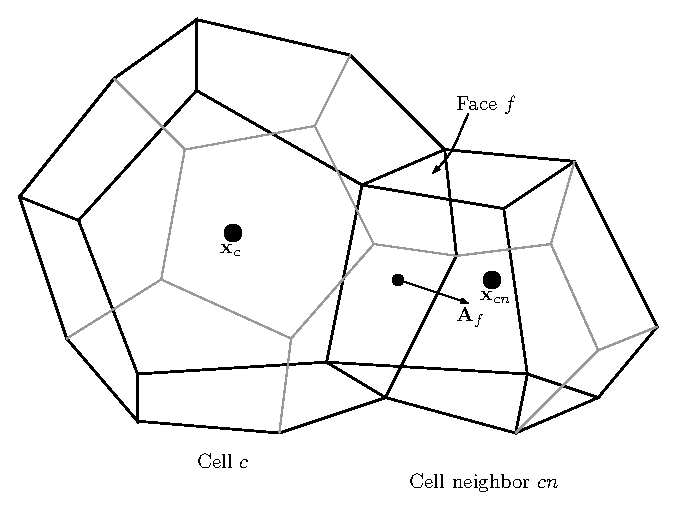
\includegraphics[width=0.5\linewidth]{figures/FaceOrientation}
\caption{Schematic of a multidimensional cell.}
\label{fig:faceorientation}
\end{figure}

\noindent
We first apply a spatial integration of Eq. \eqref{eq:euler_operator_form} over the finite volume of a cell,
\beqn 
\int_V \biggr( 
\partialderiv{\mathbf{U}}{t} + 
\bnabla \dotp \mathcal{F}(\mathbf{U})
\biggr) dV &= 
\int_V \mathbf{Q} dV \\
\eeqn 
where $\mathcal{F} (\mathbf{U}) = \big[
\mathbf{F}(\mathbf{U}),
\mathbf{G}(\mathbf{U}), 
\mathbf{H}(\mathbf{U})
\big]$. Next, using Gauss's divergence theorem, allows us to write
\beqn
\int_V \partialderiv{\mathbf{U}}{t}  dV 
+ 
\int_S \mathbf{n} \dotp \mathcal{F}  dA &= 
\int_V \mathbf{Q} dV .
\eeqn 
Now, using cell $c$ as the volume of integration, and assuming $\mathbf{U}$ and $\mathbf{Q}$ constant over the cell, with values $\mathbf{U}_c$ and $\mathbf{Q}_c$, the above equation becomes
\beqn \label{eq:general_finite_volume}
V_c \partialderiv{\mathbf{U}_c}{t} 
+ 
\sum_{f=0}^{N_{f,c}{-}1} 
\mathbf{A}_f \dotp \mathcal{F}_f
= 
V_c \mathbf{Q}_c.
\eeqn 
where $V_c$ is the volume of the cell, $N_{f,c}$ is the number of faces for cell $c$, $\mathbf{A}_f$ is the area-vector of face $f$, which is the product of the face area, $A_f$, and the face normal, $\mathbf{n}_f$ (i.e., $\mathbf{A}_f = A_f \mathbf{n}_f$), and $\mathcal{F}_f = \mathcal{F}(\mathbf{U}_f)$ is the face flux vector.  The treatment of the $\mathcal{F}_f$ term is the topic of the MUSCL-Hancock method which we detail in section \ref{section:MHM}.

\vspace{1cm}
\subsection{Multidimensional transformation of interface fluxes} \label{section:3dtransformation}
Most of the Riemann solver schemes presented in \cite{Toro} are for one dimensional geometries. A transformation technique is prescribed in \cite{Toro}, using the rotational-invariant property of the fluid flow, that allows one to use the one dimensional formulations.

Given the arbitrary face area vector, $\mathbf{A}_f=\mathbf{n}_f A_f$, we first seek a rotation matrix, $R_{\ihat}$, to rotate any vector about an axis $\mathbf{a}_{\ihat}$ such that it is aligned with $\ihat$. To determine $R_{\ihat}$ we first set the rotation axis as
\beqn 
\mathbf{a}_{\ihat} = 
\begin{cases}
\dfrac{\mathbf{n}_f \times \ihat}{||\mathbf{n}_f \times \ihat||}, &\text{ if } \mathbf{n_f}\dotp \ihat < 1{-}\epsilon \\
\jhat, &\text{ if } \mathbf{n_f}\dotp \ihat \ge 1{-}\epsilon
\end{cases}
\eeqn 
and the angle of rotation, $\theta_{\ihat}$, as
\beqn 
\theta_{\ihat} = \arccos (\mathbf{n}_f \dotp \ihat).
\eeqn 
We then apply Rodrigues's formula as detailed in appendix \ref{appendix:Roderigues_formula} to obtain $R_{\ihat}$, the associated rotation matrix. With this matrix in hand we can form the general transformation matrix, $T_{\ihat}$, defined as
\beqn
T_{\ihat} = \text{diag}(1,R,1) = 
\begin{bmatrix}
1 & 0         & 0         & 0         & 0 \\
0 & R_{00} & R_{01} & R_{02} & 0 \\
0 & R_{10} & R_{11} & R_{12} & 0 \\
0 & R_{20} & R_{21} & R_{22} & 0 \\
0 & 0         & 0         & 0         & 1 \\
\end{bmatrix}
\eeqn
which can be used to define 
\beqn 
\hatbf{F} (\mathbf{U})= \mathbf{F}(T_{\ihat} \mathbf{U})
\eeqn 
such that
\beqn 
\mathbf{n}_f \dotp \mathcal{F}_f
= \mathbf{n} \dotp [
\mathbf{F}(\mathbf{U}_f),
\mathbf{G}(\mathbf{U}_f),
\mathbf{H}(\mathbf{U}_f)]
=
T_{\ihat}^{-1} \hatbf{F}_f
\eeqn 
where we also define
\beqn 
\mathbf{F}^*(\mathbf{U}) = T_{\ihat}^{-1} \hatbf{F} (\mathbf{U})
\eeqn 
allowing us to write Eq. \eqref{eq:general_finite_volume} as 
\beqn 
\partialderiv{\mathbf{U}_c}{t} 
+ 
\frac{1}{V_c}
\sum_{f=0}^{N_{f,c}{-}1} 
A_f  \mathbf{F}_f^*
=  \mathbf{Q}_c.
\eeqn 
In this form any Riemann solver can simply be supplied with $\mathbf{U}$ for the cells on either side of an interface, and the face normal, $\mathbf{n}_f$, in order to use the classical one dimensional formulations contained in \cite{Toro}. The given Riemann solver will then produce the appropriate value for $\mathbf{F}_f^*$.



%\vspace{1cm}
%\subsection{One dimensional Finite Volume discretization}
%In one dimension we will be using the indexing scheme as shown in Figure \ref{fig:mesh1d} below. Cell indices are $i\in[0, N_c-1]$ where $N_c$ is the number of cells in the problem. The indices also indicate a cell's position from left to right, $i{=}0$ denoting the left-most cell and $i{=}N_c{-1}$ denoting the right-most cell. Throughout this research we will also use \textit{virtual nodes} to indicate the interfaces between cells, these will be denoted with half indices, i.e., $i{=}\frac{1}{2}$ denotes the interface between cell $i=0$ and cell $i=1$.
%\begin{figure}[H]
%\centering
%\includegraphics[width=1.0\linewidth]{figures/Mesh1D}
%\caption{One dimensional mesh description.}
%\label{fig:mesh1d}
%\end{figure}
%Using this indexing scheme allows us to write Eq. \eqref{eq:general_finite_volume} as
%\beqn 
%\partialderiv{\mathbf{U}_i}{t} + \frac{\ihat}{\Delta x_i}  \dotp
%\biggr(
%\mathbf{F}_{i{+}\frac{1}{2}} - \mathbf{F}_{i{-}\frac{1}{2}}
%\biggr)
%= \mathbf{Q}_i
%\eeqn 
%where $\mathbf{F}_{i{+}\frac{1}{2}}$ and $\mathbf{F}_{i{-}\frac{1}{2}}$ are now the interface flux terms and are not yet defined. The definition of these interface fluxes is the topic of next section.


\vspace{1cm}
\section{MUSCL-Hancock Method (MHM)} \label{section:MHM}
The MUSCL-Hancock method is conceptually simple. It prescribes how the interface fluxes are to be computed at the beginning of a time step and then how to supply the necessary inputs to a Riemann-solver for the computation of the preserved variables at the end of the timestep.

MUSCL stands for Monotone Upstream-centered Scheme for Conservation Laws. The scheme as modified by S. Hancock gives the method its name. We will refer to this method by using the abbreviation $MHM$.
\newline
\newline
\noindent
A single time step using MHM involves four basic steps.

\subsection{Step 1 - Compute the maximum timestep}
Generally, the time step size, $\Delta t$, needs to be limited in order to ensure numerical stability. The Courant-Friedrichs-Lewy (CFL) condition is the ratio
\beqn 
\frac{||\mathbf{u}|| \Delta t}{L_c} \le CFL,
\eeqn 
where $L_c$ is the characteristic length of cell $c$ and the value of $CFL$ is subject to the relevant numerical scheme under consideration. For explicit schemes the value of $CFL$ is generally less than 1. When $CFL=1$ the above expression indicates that the distance traveled by a unit of information, traveling at a velocity $\mathbf{u}$, over a time period $\Delta t$, cannot exceed the length of a cell. 

By specifying the value of $CFL$ the CFL-limited time step size for cell $c$, $\Delta t_{hydro,c}$, is then
\beqn 
\Delta t_{hydro,c} = \frac{CFL \ L_c}{||\mathbf{u}||}
\eeqn 
where $||\mathbf{u}||$ has not yet been resolved. One option for $\mathbf{u}$ is to use the maximum possible wave speed based on the velocity and sound speed in cell $c$, $\mathbf{u}_c$ and $a_c$ respectively, as
\beqn 
||\mathbf{u}||= ||\mathbf{u}_c|| + a_c,
\eeqn
where
\beqn 
a_c = \sqrt{\frac{\gamma_c p_c}{\rho_c}}.
\eeqn 
The simulation time-step size-limit, $\Delta t_{hydro}$, is then 
\beqn 
\Delta t_{hydro} = \min_c \biggr(\Delta t_{hydro,c}\biggr).
\eeqn 

For finer control of the simulation the user may also specify a maximum time step size, $\Delta t_{max}$. Finally, the simulation time step size, $\Delta t$, is then
\beqn 
\Delta t = \max \biggr( \Delta t_{max}, \Delta t_{hydro}\biggr).
\eeqn 


\subsection{Step 2 - Estimate the gradient $\bnabla \mathbf{U}$}
Provided that an orthogonal mush is used, the gradient can be estimated in each cell $c$ from
\beqn \label{eq:gradient}
\big\{ \bnabla \mathbf{U} \big\}_c^n
\approx
\frac{1}{V_c}
\sum_{f=0}^{N_{f,c}{-1}}  
\biggr\{
\mathbf{A}_f \otimes
\biggr(
\frac{||\position_f - \position_c||}{||\position_{cn} - \position_c||} \mathbf{U}_c^n
+
\frac{||\position_c - \position_f||}{||\position_{cn} - \position_c||} \mathbf{U}_{cn}^n
\biggr)
\biggr\},
\eeqn 
where $V_c$ is the volume of cell $c$, $N_{f,c}$ is the number of faces for cell $c$, $A_f$ the face area-vector of face $f$ (i.e., $\mathbf{A}_f = A_f \mathbf{n}_f$), $\position_{cn}$ is the centroid of the neighboring cell $cn$ at face $f$, and finally $\mathbf{U}_{cn}$ is the finite volume cell-constant value of $\mathbf{U}$ for cell $cn$. For non-orthogonal meshes the gradient can be corrected as shown in \cite{Moukalled}.
\newline 
\newline
\textbf{Limiting:}\newline
The cell-wise gradients computed in Eq. \eqref{eq:gradient} requires limiting to avoid numerical oscillations. The chosen limiting scheme, to ensure specific properties when coupled with radiation transport (i.e., asymptotic diffusion limit), is the double minmod limiter, as prescribed in \cite{McClarrenSlopes}. The definition of the double minmod limiter in \cite{McClarrenSlopes} is either misleading or incorrectly defined as it implies that all gradients are limited to $\ge 0$, therefore we define this limiter in detail here based on the cited literature of \cite{McClarrenSlopes}.

The \textbf{general vector-based minmod limiter}, for an $M$ amount of vectors with each vector having $N$ elements, is defined as
\beqn
\text{minmod}(\mathbf{U}^0, \dots, \mathbf{U}^{M-1}) = 
\begin{bmatrix}
	\text{minmod}(U_0^0, \dots, U_0^{M-1}) \\
	\vdots \\
	\text{minmod}(U_{N-1}^0, \dots, U_{N-1}^{M-1})
\end{bmatrix},
\eeqn 
where $U_n^m$ denotes the $n$-th entry of the $m$-th vector. The \textbf{general scalar-based minmod limiter}, for $M$ amount of scalar elements, is defined as
\beqn 
\text{minmod}(c_0, \dots, c_{M-1}) = 
\begin{cases}
	0, &\text{ if } \text{sign}(a_0) \ne  \text{sign}(a_m) \text{ for any } m \\
	\min(a_0, \dots, a_{M-1}), &\text{ if } a_m > 0 \text{ for all } m \\
	\max(a_0, \dots, a_{M-1}), &\text{ if } a_m < 0 \text{ for all } m \\
\end{cases}.
\eeqn 
These two general limiters are used to define the \textbf{double minmod limiter} for the gradient of cell $c$, which has $M$ amount of neighbor cells.
\beqn 
\text{double minmod limited }\big\{ \bnabla \mathbf{U} \big\}_c^n = 
	\text{minmod}\biggr(
	\big\{ \bnabla \mathbf{U} \big\}_{c}^n,
	\alpha \bigg\{ \position_{ccn,x} \otimes
	\dfrac{\mathbf{U}_{cn} - \mathbf{U}_c}{||\position_{ccn}||^2} \bigg\} \text{ for all } cn\in[0,M-1]
	\biggr) 
\eeqn 
where $\position_{ccn} = \position_{cn} - \position_c$ and $\alpha{=2}$ denoting the ``double''. When $\alpha{=0}$ the scheme reduces to the unlimited scheme and if $\alpha{=1}$ the scheme is the standard minmod limiter.

\newpage
\subsection{Step 3 - Advance the conserved variables by half a time step}
Advance the cell-centered values over half a time step as
\beqn 
\mathbf{U}_c^{n{+}\frac{1}{2}} = \mathbf{U}_c^n - \frac{\frac{1}{2}\Delta t^n}{V_c} \sum_{f=0}^{N_{f,c}{-1}} 
\biggr(
A_f \mathbf{F}_f^{*n}
\biggr)
+ \frac{1}{2}\Delta t^n \mathbf{Q}.
\eeqn 
where $\mathbf{F}_f^{*n} = \mathbf{F}^*(\mathbf{U}_f^n) $. $\mathbf{U}_f^n$ is extrapolated from $\mathbf{U}_c^n$ as
\beqn 
\mathbf{U}_f^{n} = \mathbf{U}_c^{n}  + (\position_{f} - \position_c) \dotp \big\{ \bnabla \mathbf{U} \big\}_c^n
\eeqn 
where $\position_f$ is the face-centroid.


\subsection{Step 4 - Execute a series of Riemann solvers}
A Riemann solver computes the interface fluxes, $\mathbf{F}_f^{*\mathcal{R},n{+}\frac{1}{2}}$, using $\mathbf{U}_c^{n{+}\frac{1}{2}}$, where $\mathcal{R}$ denotes the specific Riemann solver. These interface fluxes are then used to advance the conserved variables by a single timestep as
\beqn 
\mathbf{U}_c^{n+1} = \mathbf{U}_c^n - \frac{\Delta t^n}{V_c} \sum_{f=0}^{N_{f,c}{-1}} 
\biggr(
A_f
\mathbf{F}_f^{*\mathcal{R},n{+}\frac{1}{2}}
\biggr)
+ \Delta t^n \mathbf{Q}.
\eeqn 
The discontinuity across a face is treated as a one dimensional problem with a left and right side having different values for $\mathbf{U}$, i.e., $\mathbf{U}_L = \mathbf{U}_{f,c}^{n{+}\frac{1}{2}}$ and $\mathbf{U}_R = \mathbf{U}_{f,cn}^{n{+}\frac{1}{2}}$ for the left and right side respectively. The face values of $\mathbf{U}$ are extrapolated using the gradient $\{\bnabla\mathbf{U}\}^n$ such that
\begin{subequations}
\begin{equation}
\mathbf{U}_{f,c}^{n} = \mathbf{U}_c^{n+\frac{1}{2}}  + (\position_{f} - \position_c) \dotp \big\{ \bnabla \mathbf{U} \big\}_c^n
\end{equation}
\begin{equation}
\mathbf{U}_{f,cn}^{n} = \mathbf{U}_{cn}^{n+\frac{1}{2}}  + (\position_{f} - \position_{cn}) \dotp \big\{ \bnabla \mathbf{U} \big\}_{cn}^n.
\end{equation}
\end{subequations}




When using the HLLC solver, as described in \cite{Toro}, the Riemann solver will compute $\mathbf{F}_f^{*hllc,n{+}\frac{1}{2}}$ after which we compute the conserved variables at $n+1$ from
\beqn 
\mathbf{U}_c^{n+1} = \mathbf{U}_c^n - \frac{\Delta t^n}{V_c} \sum_{f=0}^{N_{f,c}{-1}} 
\biggr(
A_f
\mathbf{F}_f^{*hllc,n{+}\frac{1}{2}}
\biggr)
+ \Delta t^n \mathbf{Q}.
\eeqn 
The HLLC Riemann solver is detailed in section \ref{section:HLLC}.

\newpage 
\section{The HLLC Approximate Riemann Solver} \label{section:HLLC}
The Harten, Lax and van Leer (HLL) solver scheme was developed in 1983 \cite{Toro} and requires estimates for the fastest wave/signal/shock velocities emerging from a discontinuity. Later Toro, Spruce and Speares proposed the Harten, Lax, van Leer, \textit{Contact} (HLLC) scheme \cite{Toro} which adds another wave to the problem.
\newline
\newline
The first input, required by the HLLC Riemann solver, is the face normal, $\mathbf{n}_f$, which allows us to compute the transformation matrix, $T_{\ihat}$, as per section \ref{section:3dtransformation}. The other input parameters are then
\beqn 
\mathbf{U}_L &= T_{\ihat} \mathbf{U}_{f,c}^{n{+}\frac{1}{2}}, \\
\mathbf{U}_R &= T_{\ihat} \mathbf{U}_{f,cn}^{n{+}\frac{1}{2}}, \\
\mathbf{F}_L &= \mathbf{F}(T_{\ihat} \mathbf{U}_{f,c}^{n{+}\frac{1}{2}}), \\
\mathbf{F}_R &= \mathbf{F}(T_{\ihat} \mathbf{U}_{f,cn}^{n{+}\frac{1}{2}}), \\
p_L &= p_c, \quad \gamma_L = \gamma_c,\\
p_R &= p_{cn}, \quad \gamma_R = \gamma_{cn},
\eeqn 
where the quantifies denoted with $c$ denotes those belonging to the cell which maintains a negative sense with respect to face $f$, and conversely $cn$ denotes the quantities associated with the cell maintaining a positive sense with respect to the face.


\subsection{Left and right wave speed estimation}
The HLLC Riemann solver is predicated on knowing an estimate for wave speeds $S_L$ and $S_R$, which we estimate as
\beqn 
S_L = \min(u_L-a_L, u_R-a_R)
\eeqn 
and
\beqn 
S_R = \max(u_L+a_L,u_R+a_R).
\eeqn 
where $a_L$ and $a_R$ are the sound speeds associated with the left- and right conserved variables as
\beqn 
a = \sqrt{\frac{\gamma p}{\rho}}.
\eeqn 
Next we require the contact wave speed.

\subsection{Contact wave speed}
The contact wave speed, $S_*$, is given by
\beqn 
S_* = \frac{p_R - p_L +\rho_L u_L(S_L-u_L) - \rho_R u_R(S_R-u_R)}
{\rho_L (S_L-u_L) - \rho_R(S_R-u_R)}.
\eeqn 

\subsection{Intermediate fluxes}
As per \cite{Toro} the intermediate fluxes, $\mathbf{F}_{*L}$ and $\mathbf{F}_{*R}$ are given by
\beqn 
F_{*K} = 
\frac
{S_* (S_K \mathbf{U}_K - \mathbf{F}_K) + S_K(p_K+\rho_L(S_K-u_K)(S_*-u_K))D_*}
{S_K - S_*}
\eeqn 
for $K=L$ and $K=R$. The vector $\mathbf{D}_*$ is a vector such that
\beqn 
\mathbf{F}(\mathbf{U}) = u \mathbf{U} + p\mathbf{D},
\eeqn 
therefore 
\beqn 
\mathbf{D}_* = [0,1,0,0,S_*]^T
\eeqn 

\subsection{Interface flux}
The interface flux $\mathbf{F}_f^{*hllc}$ is now given by
\beqn 
\mathbf{F}_f^{*hllc} &= 
T_{\ihat}^{-1} \mathbf{F}_f^{hllc}  \\
\mathbf{F}_f^{hllc} &= 
\begin{cases}
\mathbf{F}_L &,\text{ if } S_L \ge 0, \\
\mathbf{F}_{*L} &,\text{ if } S_L \le 0 \le S_*, \\
\mathbf{F}_{*R} &,\text{ if } S_* \le 0 \le S_R, \\
\mathbf{F}_R &,\text{ if } S_R \le 0
\end{cases}
\eeqn 

\vspace{1cm}
\section{Verification - Sod shock tube problem}
The Sod shock tube problem is a simple problem with the following specifications:
\begin{itemize}
	\item The one dimensional problem domain has a total size of 1.0 spanning $x\in[-\frac{1}{2},\frac{1}{2}]$.
	\item The left-half of the problem has an initial state denoted with $L$ and the right-half has an initial state denoted with $R$.
	\item At time $t=0$:
	\begin{itemize}
		\item Densities: $\rho_L = 1$, $\rho_R = 0.125$
		\item Pressures: $p_L=1$, $p_R=0.1$
		\item Velocity: $u=0 \ \forall x$  
		\item Ratio of specific heats: $\gamma=1.4 \ \forall x$
		\item Boundary conditions: Transmissive
	\end{itemize} 
\end{itemize}

As time evolves the problem exhibits a shock-wave, a contact-wave and a rarefaction-wave. The analytical solution has been obtain from a Fortran code by Timmers \cite{Timmers}. At time $t=0.2$ the analytical solution for $\rho$, $p$, $u$ and $e$ is tabulated over 500 points in appendix \ref{appendix:sodanasol}.

The MHM-HLLC scheme employed above has been executed with the following inputs:
\begin{itemize}
	\item $\Delta t_{max}=1e-2$
	\item $CFL=0.3$
	\item Maximum number of timesteps, $2000$
	\item Maximum total time, $0.2$
	\item $\Delta x=0.01$ or 100 cells.
\end{itemize}
The program reached the maximum total time after 73 iterations and the results at $t=0.2$ is compared to the analytical solution in Figure \ref{fig:compinfflow1dtest1output}.

\begin{figure}[H]
	\centering
	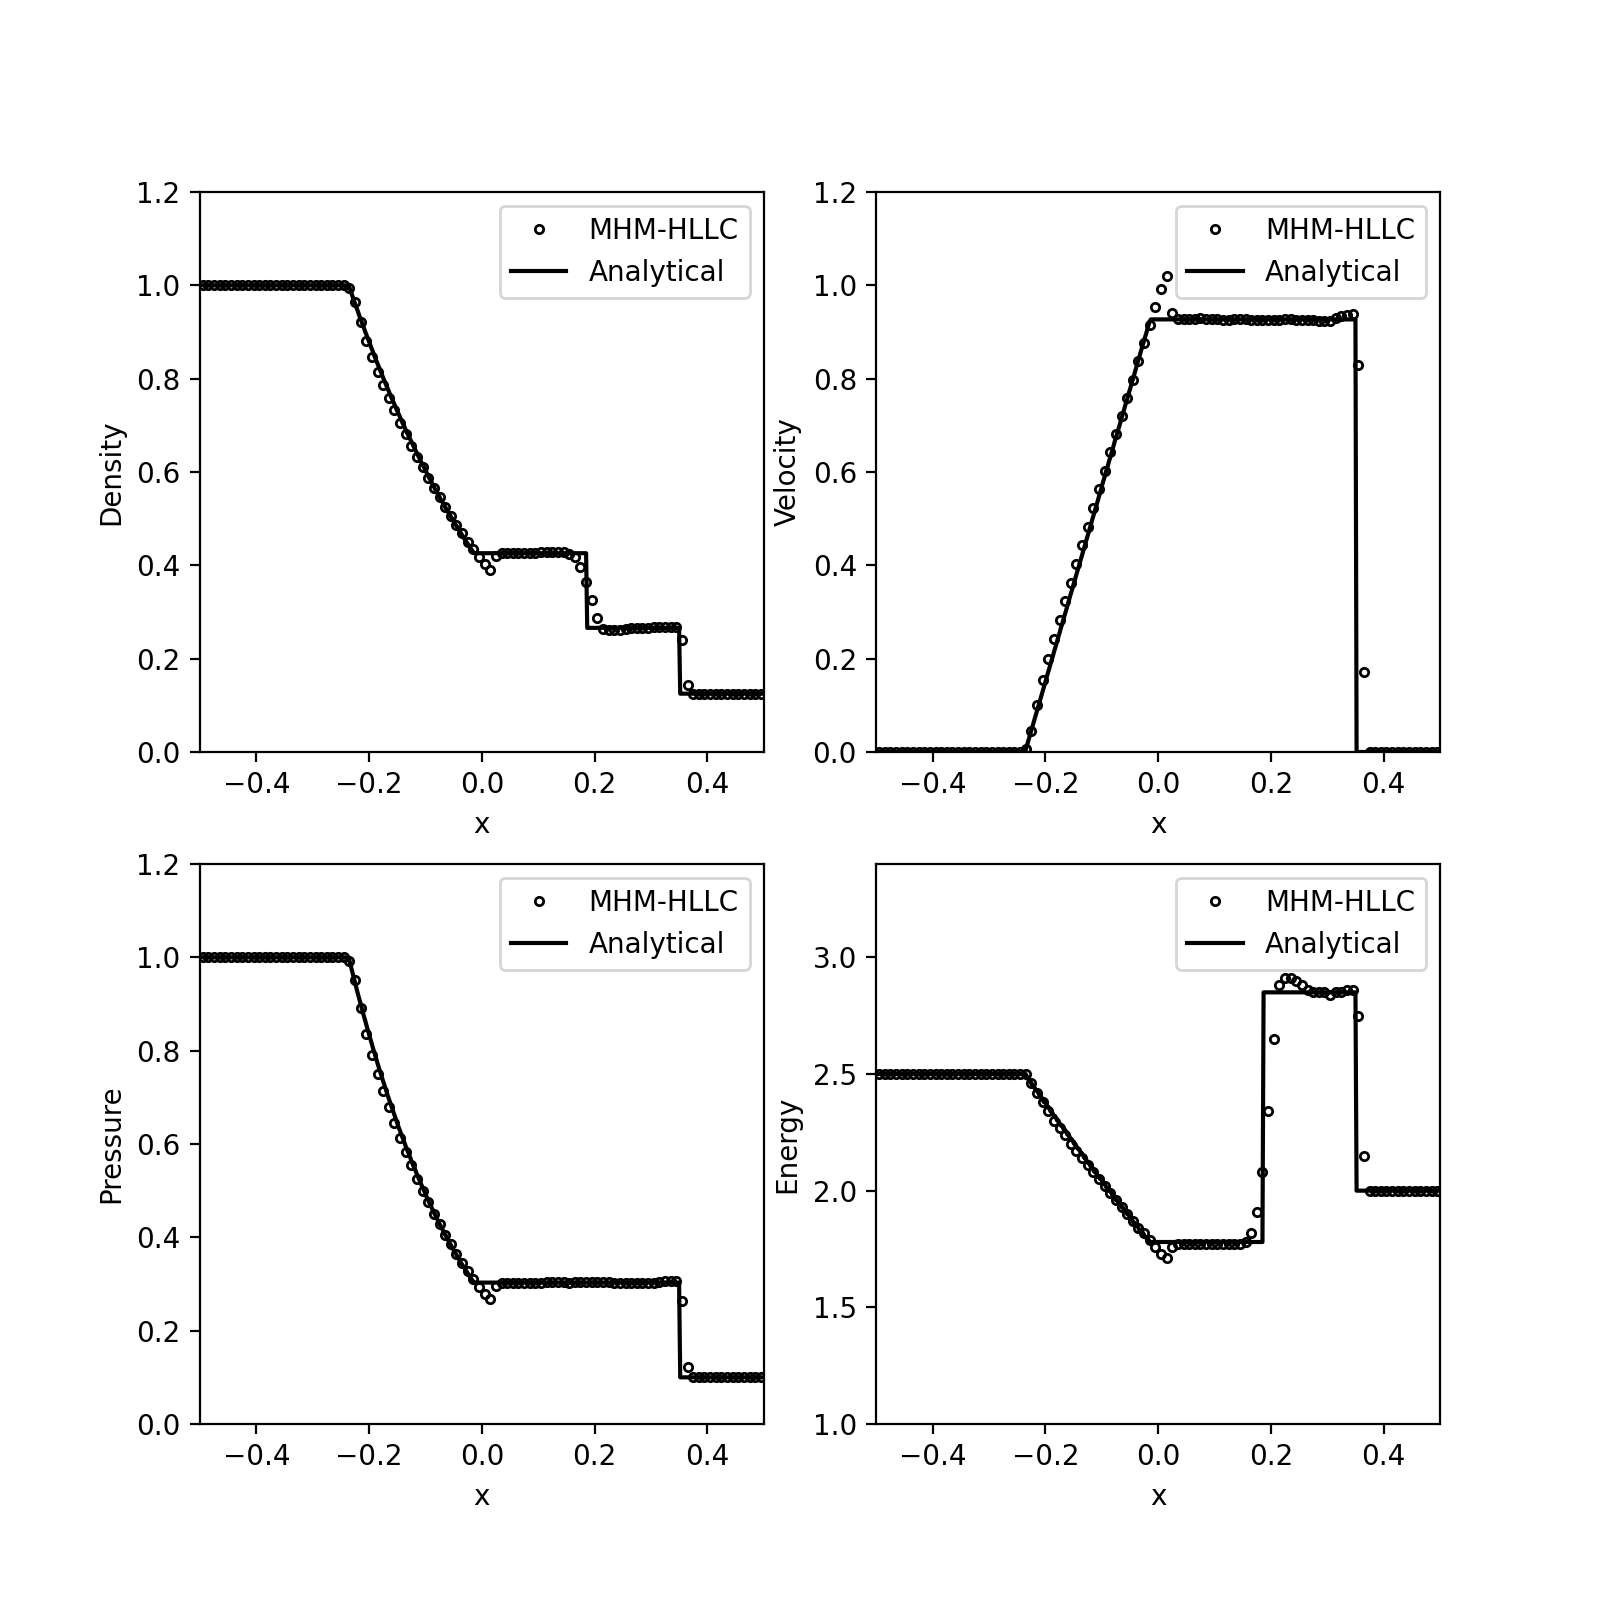
\includegraphics[width=1.0\linewidth]{figures/CompInFFlow1D_Test1_output.png}
	\caption{Numerical results compared to the analytical results at $t=0.2$.}
	\label{fig:compinfflow1dtest1output}
\end{figure}


\newpage
\begin{thebibliography}{1}
	
%	\bibitem{LewisMiller} Lewis E.E., Miller W.F., {\em Computational Methods of Neutron Transport}, JohnWiley \& Sons, 1984
	
	\bibitem{Toro} Toro E.F., {\em Riemann Solvers and Numerical Methods for Fluid Dynamics - A Practical Introduction}, third edition, Springer, 2009.
	
	\bibitem{Moukalled} Moukalled F.,  Mangani L., Darwish M., {\em The Finite Volume Method in Computational Fluid Dynamics - An Advanced Introduction withOpenFOAM® and Matlab®}, Springer, 2016.
	
	\bibitem{McClarrenSlopes} McClarren R.G., Lowrie R.B., {\em The effects of slope limiting on asymptotic-preserving numerical methods for hyperbolic conservation laws}, Journal of Computational Physics, vol 227 p9711-9726, 2008.
	
	\bibitem{Timmers} Timmers F.X., {\em Exact Riemann Solver}, Website: https://cococubed.com/code\_pages/exact\_riemann.shtml, accessed April 22, 2022.
	
	   
\end{thebibliography}

\newpage
\begin{appendices}
\section{Roderigues's formula} \label{appendix:Roderigues_formula}
Roderigues' formula for the rotation of a vector $\mathbf{v}$ about a unit vector $\mathbf{a}$ with right-hand rule
\begin{equation}
\newcommand{\vvec}{\mathbf{v}}
\newcommand{\avec}{\mathbf{a}}
\begin{aligned}
\vvec_{rotated} &= \cos \theta \vvec + (\avec \dotp \vvec)(1-\cos \theta) \avec + \sin \theta (\avec \times \vvec)
\end{aligned}
\end{equation}
In matrix form
\beqn 
\mathbf{v}_{rotated} = A \mathbf{v}
\eeqn 
where
\beqn 
A = 
\begin{bmatrix}
0 & -a_z & a_y \\
a_z & 0 & -a_x \\
-a_y & a_x & 0
\end{bmatrix}
\eeqn 
and
\beqn 
R = I + \sin\theta A + (1-\cos\theta) A^2
\eeqn


\section{Sod shock tube problem - analytical solution at $t=0.2$} \label{appendix:sodanasol}
{\scriptsize 
\begin{verbatim}
   i           x    density     pressure    velocity    energy      i           x    density     pressure    velocity    energy 
   1   -5.00E-01    1.00E+00    1.00E+00    0.00E+00    2.50E+00  251    1.00E-03    4.26E-01    3.03E-01    9.27E-01    1.78E+00
   2   -4.98E-01    1.00E+00    1.00E+00    0.00E+00    2.50E+00  252    3.01E-03    4.26E-01    3.03E-01    9.27E-01    1.78E+00
   3   -4.96E-01    1.00E+00    1.00E+00    0.00E+00    2.50E+00  253    5.01E-03    4.26E-01    3.03E-01    9.27E-01    1.78E+00
   4   -4.94E-01    1.00E+00    1.00E+00    0.00E+00    2.50E+00  254    7.01E-03    4.26E-01    3.03E-01    9.27E-01    1.78E+00
   5   -4.92E-01    1.00E+00    1.00E+00    0.00E+00    2.50E+00  255    9.02E-03    4.26E-01    3.03E-01    9.27E-01    1.78E+00
   6   -4.90E-01    1.00E+00    1.00E+00    0.00E+00    2.50E+00  256    1.10E-02    4.26E-01    3.03E-01    9.27E-01    1.78E+00
   7   -4.88E-01    1.00E+00    1.00E+00    0.00E+00    2.50E+00  257    1.30E-02    4.26E-01    3.03E-01    9.27E-01    1.78E+00
   8   -4.86E-01    1.00E+00    1.00E+00    0.00E+00    2.50E+00  258    1.50E-02    4.26E-01    3.03E-01    9.27E-01    1.78E+00
   9   -4.84E-01    1.00E+00    1.00E+00    0.00E+00    2.50E+00  259    1.70E-02    4.26E-01    3.03E-01    9.27E-01    1.78E+00
  10   -4.82E-01    1.00E+00    1.00E+00    0.00E+00    2.50E+00  260    1.90E-02    4.26E-01    3.03E-01    9.27E-01    1.78E+00
  11   -4.80E-01    1.00E+00    1.00E+00    0.00E+00    2.50E+00  261    2.10E-02    4.26E-01    3.03E-01    9.27E-01    1.78E+00
  12   -4.78E-01    1.00E+00    1.00E+00    0.00E+00    2.50E+00  262    2.30E-02    4.26E-01    3.03E-01    9.27E-01    1.78E+00
  13   -4.76E-01    1.00E+00    1.00E+00    0.00E+00    2.50E+00  263    2.51E-02    4.26E-01    3.03E-01    9.27E-01    1.78E+00
  14   -4.74E-01    1.00E+00    1.00E+00    0.00E+00    2.50E+00  264    2.71E-02    4.26E-01    3.03E-01    9.27E-01    1.78E+00
  15   -4.72E-01    1.00E+00    1.00E+00    0.00E+00    2.50E+00  265    2.91E-02    4.26E-01    3.03E-01    9.27E-01    1.78E+00
  16   -4.70E-01    1.00E+00    1.00E+00    0.00E+00    2.50E+00  266    3.11E-02    4.26E-01    3.03E-01    9.27E-01    1.78E+00
  17   -4.68E-01    1.00E+00    1.00E+00    0.00E+00    2.50E+00  267    3.31E-02    4.26E-01    3.03E-01    9.27E-01    1.78E+00
  18   -4.66E-01    1.00E+00    1.00E+00    0.00E+00    2.50E+00  268    3.51E-02    4.26E-01    3.03E-01    9.27E-01    1.78E+00
  19   -4.64E-01    1.00E+00    1.00E+00    0.00E+00    2.50E+00  269    3.71E-02    4.26E-01    3.03E-01    9.27E-01    1.78E+00
  20   -4.62E-01    1.00E+00    1.00E+00    0.00E+00    2.50E+00  270    3.91E-02    4.26E-01    3.03E-01    9.27E-01    1.78E+00
  21   -4.60E-01    1.00E+00    1.00E+00    0.00E+00    2.50E+00  271    4.11E-02    4.26E-01    3.03E-01    9.27E-01    1.78E+00
  22   -4.58E-01    1.00E+00    1.00E+00    0.00E+00    2.50E+00  272    4.31E-02    4.26E-01    3.03E-01    9.27E-01    1.78E+00
  23   -4.56E-01    1.00E+00    1.00E+00    0.00E+00    2.50E+00  273    4.51E-02    4.26E-01    3.03E-01    9.27E-01    1.78E+00
  24   -4.54E-01    1.00E+00    1.00E+00    0.00E+00    2.50E+00  274    4.71E-02    4.26E-01    3.03E-01    9.27E-01    1.78E+00
  25   -4.52E-01    1.00E+00    1.00E+00    0.00E+00    2.50E+00  275    4.91E-02    4.26E-01    3.03E-01    9.27E-01    1.78E+00
  26   -4.50E-01    1.00E+00    1.00E+00    0.00E+00    2.50E+00  276    5.11E-02    4.26E-01    3.03E-01    9.27E-01    1.78E+00
  27   -4.48E-01    1.00E+00    1.00E+00    0.00E+00    2.50E+00  277    5.31E-02    4.26E-01    3.03E-01    9.27E-01    1.78E+00
  28   -4.46E-01    1.00E+00    1.00E+00    0.00E+00    2.50E+00  278    5.51E-02    4.26E-01    3.03E-01    9.27E-01    1.78E+00
  29   -4.44E-01    1.00E+00    1.00E+00    0.00E+00    2.50E+00  279    5.71E-02    4.26E-01    3.03E-01    9.27E-01    1.78E+00
  30   -4.42E-01    1.00E+00    1.00E+00    0.00E+00    2.50E+00  280    5.91E-02    4.26E-01    3.03E-01    9.27E-01    1.78E+00
  31   -4.40E-01    1.00E+00    1.00E+00    0.00E+00    2.50E+00  281    6.11E-02    4.26E-01    3.03E-01    9.27E-01    1.78E+00
  32   -4.38E-01    1.00E+00    1.00E+00    0.00E+00    2.50E+00  282    6.31E-02    4.26E-01    3.03E-01    9.27E-01    1.78E+00
  33   -4.36E-01    1.00E+00    1.00E+00    0.00E+00    2.50E+00  283    6.51E-02    4.26E-01    3.03E-01    9.27E-01    1.78E+00
  34   -4.34E-01    1.00E+00    1.00E+00    0.00E+00    2.50E+00  284    6.71E-02    4.26E-01    3.03E-01    9.27E-01    1.78E+00
  35   -4.32E-01    1.00E+00    1.00E+00    0.00E+00    2.50E+00  285    6.91E-02    4.26E-01    3.03E-01    9.27E-01    1.78E+00
  36   -4.30E-01    1.00E+00    1.00E+00    0.00E+00    2.50E+00  286    7.11E-02    4.26E-01    3.03E-01    9.27E-01    1.78E+00
  37   -4.28E-01    1.00E+00    1.00E+00    0.00E+00    2.50E+00  287    7.31E-02    4.26E-01    3.03E-01    9.27E-01    1.78E+00
  38   -4.26E-01    1.00E+00    1.00E+00    0.00E+00    2.50E+00  288    7.52E-02    4.26E-01    3.03E-01    9.27E-01    1.78E+00
  39   -4.24E-01    1.00E+00    1.00E+00    0.00E+00    2.50E+00  289    7.72E-02    4.26E-01    3.03E-01    9.27E-01    1.78E+00
  40   -4.22E-01    1.00E+00    1.00E+00    0.00E+00    2.50E+00  290    7.92E-02    4.26E-01    3.03E-01    9.27E-01    1.78E+00
  41   -4.20E-01    1.00E+00    1.00E+00    0.00E+00    2.50E+00  291    8.12E-02    4.26E-01    3.03E-01    9.27E-01    1.78E+00
  42   -4.18E-01    1.00E+00    1.00E+00    0.00E+00    2.50E+00  292    8.32E-02    4.26E-01    3.03E-01    9.27E-01    1.78E+00
  43   -4.16E-01    1.00E+00    1.00E+00    0.00E+00    2.50E+00  293    8.52E-02    4.26E-01    3.03E-01    9.27E-01    1.78E+00
  44   -4.14E-01    1.00E+00    1.00E+00    0.00E+00    2.50E+00  294    8.72E-02    4.26E-01    3.03E-01    9.27E-01    1.78E+00
  45   -4.12E-01    1.00E+00    1.00E+00    0.00E+00    2.50E+00  295    8.92E-02    4.26E-01    3.03E-01    9.27E-01    1.78E+00
  46   -4.10E-01    1.00E+00    1.00E+00    0.00E+00    2.50E+00  296    9.12E-02    4.26E-01    3.03E-01    9.27E-01    1.78E+00
  47   -4.08E-01    1.00E+00    1.00E+00    0.00E+00    2.50E+00  297    9.32E-02    4.26E-01    3.03E-01    9.27E-01    1.78E+00
  48   -4.06E-01    1.00E+00    1.00E+00    0.00E+00    2.50E+00  298    9.52E-02    4.26E-01    3.03E-01    9.27E-01    1.78E+00
  49   -4.04E-01    1.00E+00    1.00E+00    0.00E+00    2.50E+00  299    9.72E-02    4.26E-01    3.03E-01    9.27E-01    1.78E+00
  50   -4.02E-01    1.00E+00    1.00E+00    0.00E+00    2.50E+00  300    9.92E-02    4.26E-01    3.03E-01    9.27E-01    1.78E+00
  51   -4.00E-01    1.00E+00    1.00E+00    0.00E+00    2.50E+00  301    1.01E-01    4.26E-01    3.03E-01    9.27E-01    1.78E+00
  52   -3.98E-01    1.00E+00    1.00E+00    0.00E+00    2.50E+00  302    1.03E-01    4.26E-01    3.03E-01    9.27E-01    1.78E+00
  53   -3.96E-01    1.00E+00    1.00E+00    0.00E+00    2.50E+00  303    1.05E-01    4.26E-01    3.03E-01    9.27E-01    1.78E+00
  54   -3.94E-01    1.00E+00    1.00E+00    0.00E+00    2.50E+00  304    1.07E-01    4.26E-01    3.03E-01    9.27E-01    1.78E+00
  55   -3.92E-01    1.00E+00    1.00E+00    0.00E+00    2.50E+00  305    1.09E-01    4.26E-01    3.03E-01    9.27E-01    1.78E+00
  56   -3.90E-01    1.00E+00    1.00E+00    0.00E+00    2.50E+00  306    1.11E-01    4.26E-01    3.03E-01    9.27E-01    1.78E+00
  57   -3.88E-01    1.00E+00    1.00E+00    0.00E+00    2.50E+00  307    1.13E-01    4.26E-01    3.03E-01    9.27E-01    1.78E+00
  58   -3.86E-01    1.00E+00    1.00E+00    0.00E+00    2.50E+00  308    1.15E-01    4.26E-01    3.03E-01    9.27E-01    1.78E+00
  59   -3.84E-01    1.00E+00    1.00E+00    0.00E+00    2.50E+00  309    1.17E-01    4.26E-01    3.03E-01    9.27E-01    1.78E+00
  60   -3.82E-01    1.00E+00    1.00E+00    0.00E+00    2.50E+00  310    1.19E-01    4.26E-01    3.03E-01    9.27E-01    1.78E+00
  61   -3.80E-01    1.00E+00    1.00E+00    0.00E+00    2.50E+00  311    1.21E-01    4.26E-01    3.03E-01    9.27E-01    1.78E+00
  62   -3.78E-01    1.00E+00    1.00E+00    0.00E+00    2.50E+00  312    1.23E-01    4.26E-01    3.03E-01    9.27E-01    1.78E+00
  63   -3.76E-01    1.00E+00    1.00E+00    0.00E+00    2.50E+00  313    1.25E-01    4.26E-01    3.03E-01    9.27E-01    1.78E+00
  64   -3.74E-01    1.00E+00    1.00E+00    0.00E+00    2.50E+00  314    1.27E-01    4.26E-01    3.03E-01    9.27E-01    1.78E+00
  65   -3.72E-01    1.00E+00    1.00E+00    0.00E+00    2.50E+00  315    1.29E-01    4.26E-01    3.03E-01    9.27E-01    1.78E+00
  66   -3.70E-01    1.00E+00    1.00E+00    0.00E+00    2.50E+00  316    1.31E-01    4.26E-01    3.03E-01    9.27E-01    1.78E+00
  67   -3.68E-01    1.00E+00    1.00E+00    0.00E+00    2.50E+00  317    1.33E-01    4.26E-01    3.03E-01    9.27E-01    1.78E+00
  68   -3.66E-01    1.00E+00    1.00E+00    0.00E+00    2.50E+00  318    1.35E-01    4.26E-01    3.03E-01    9.27E-01    1.78E+00
  69   -3.64E-01    1.00E+00    1.00E+00    0.00E+00    2.50E+00  319    1.37E-01    4.26E-01    3.03E-01    9.27E-01    1.78E+00
  70   -3.62E-01    1.00E+00    1.00E+00    0.00E+00    2.50E+00  320    1.39E-01    4.26E-01    3.03E-01    9.27E-01    1.78E+00
  71   -3.60E-01    1.00E+00    1.00E+00    0.00E+00    2.50E+00  321    1.41E-01    4.26E-01    3.03E-01    9.27E-01    1.78E+00
  72   -3.58E-01    1.00E+00    1.00E+00    0.00E+00    2.50E+00  322    1.43E-01    4.26E-01    3.03E-01    9.27E-01    1.78E+00
  73   -3.56E-01    1.00E+00    1.00E+00    0.00E+00    2.50E+00  323    1.45E-01    4.26E-01    3.03E-01    9.27E-01    1.78E+00
  74   -3.54E-01    1.00E+00    1.00E+00    0.00E+00    2.50E+00  324    1.47E-01    4.26E-01    3.03E-01    9.27E-01    1.78E+00
  75   -3.52E-01    1.00E+00    1.00E+00    0.00E+00    2.50E+00  325    1.49E-01    4.26E-01    3.03E-01    9.27E-01    1.78E+00
  76   -3.50E-01    1.00E+00    1.00E+00    0.00E+00    2.50E+00  326    1.51E-01    4.26E-01    3.03E-01    9.27E-01    1.78E+00
  77   -3.48E-01    1.00E+00    1.00E+00    0.00E+00    2.50E+00  327    1.53E-01    4.26E-01    3.03E-01    9.27E-01    1.78E+00
  78   -3.46E-01    1.00E+00    1.00E+00    0.00E+00    2.50E+00  328    1.55E-01    4.26E-01    3.03E-01    9.27E-01    1.78E+00
  79   -3.44E-01    1.00E+00    1.00E+00    0.00E+00    2.50E+00  329    1.57E-01    4.26E-01    3.03E-01    9.27E-01    1.78E+00
  80   -3.42E-01    1.00E+00    1.00E+00    0.00E+00    2.50E+00  330    1.59E-01    4.26E-01    3.03E-01    9.27E-01    1.78E+00
  81   -3.40E-01    1.00E+00    1.00E+00    0.00E+00    2.50E+00  331    1.61E-01    4.26E-01    3.03E-01    9.27E-01    1.78E+00
  82   -3.38E-01    1.00E+00    1.00E+00    0.00E+00    2.50E+00  332    1.63E-01    4.26E-01    3.03E-01    9.27E-01    1.78E+00
  83   -3.36E-01    1.00E+00    1.00E+00    0.00E+00    2.50E+00  333    1.65E-01    4.26E-01    3.03E-01    9.27E-01    1.78E+00
  84   -3.34E-01    1.00E+00    1.00E+00    0.00E+00    2.50E+00  334    1.67E-01    4.26E-01    3.03E-01    9.27E-01    1.78E+00
  85   -3.32E-01    1.00E+00    1.00E+00    0.00E+00    2.50E+00  335    1.69E-01    4.26E-01    3.03E-01    9.27E-01    1.78E+00
  86   -3.30E-01    1.00E+00    1.00E+00    0.00E+00    2.50E+00  336    1.71E-01    4.26E-01    3.03E-01    9.27E-01    1.78E+00
  87   -3.28E-01    1.00E+00    1.00E+00    0.00E+00    2.50E+00  337    1.73E-01    4.26E-01    3.03E-01    9.27E-01    1.78E+00
  88   -3.26E-01    1.00E+00    1.00E+00    0.00E+00    2.50E+00  338    1.75E-01    4.26E-01    3.03E-01    9.27E-01    1.78E+00
  89   -3.24E-01    1.00E+00    1.00E+00    0.00E+00    2.50E+00  339    1.77E-01    4.26E-01    3.03E-01    9.27E-01    1.78E+00
  90   -3.22E-01    1.00E+00    1.00E+00    0.00E+00    2.50E+00  340    1.79E-01    4.26E-01    3.03E-01    9.27E-01    1.78E+00
  91   -3.20E-01    1.00E+00    1.00E+00    0.00E+00    2.50E+00  341    1.81E-01    4.26E-01    3.03E-01    9.27E-01    1.78E+00
  92   -3.18E-01    1.00E+00    1.00E+00    0.00E+00    2.50E+00  342    1.83E-01    4.26E-01    3.03E-01    9.27E-01    1.78E+00
  93   -3.16E-01    1.00E+00    1.00E+00    0.00E+00    2.50E+00  343    1.85E-01    4.26E-01    3.03E-01    9.27E-01    1.78E+00
  94   -3.14E-01    1.00E+00    1.00E+00    0.00E+00    2.50E+00  344    1.87E-01    2.66E-01    3.03E-01    9.27E-01    2.85E+00
  95   -3.12E-01    1.00E+00    1.00E+00    0.00E+00    2.50E+00  345    1.89E-01    2.66E-01    3.03E-01    9.27E-01    2.85E+00
  96   -3.10E-01    1.00E+00    1.00E+00    0.00E+00    2.50E+00  346    1.91E-01    2.66E-01    3.03E-01    9.27E-01    2.85E+00
  97   -3.08E-01    1.00E+00    1.00E+00    0.00E+00    2.50E+00  347    1.93E-01    2.66E-01    3.03E-01    9.27E-01    2.85E+00
  98   -3.06E-01    1.00E+00    1.00E+00    0.00E+00    2.50E+00  348    1.95E-01    2.66E-01    3.03E-01    9.27E-01    2.85E+00
  99   -3.04E-01    1.00E+00    1.00E+00    0.00E+00    2.50E+00  349    1.97E-01    2.66E-01    3.03E-01    9.27E-01    2.85E+00
 100   -3.02E-01    1.00E+00    1.00E+00    0.00E+00    2.50E+00  350    1.99E-01    2.66E-01    3.03E-01    9.27E-01    2.85E+00
 101   -3.00E-01    1.00E+00    1.00E+00    0.00E+00    2.50E+00  351    2.01E-01    2.66E-01    3.03E-01    9.27E-01    2.85E+00
 102   -2.98E-01    1.00E+00    1.00E+00    0.00E+00    2.50E+00  352    2.03E-01    2.66E-01    3.03E-01    9.27E-01    2.85E+00
 103   -2.96E-01    1.00E+00    1.00E+00    0.00E+00    2.50E+00  353    2.05E-01    2.66E-01    3.03E-01    9.27E-01    2.85E+00
 104   -2.94E-01    1.00E+00    1.00E+00    0.00E+00    2.50E+00  354    2.07E-01    2.66E-01    3.03E-01    9.27E-01    2.85E+00
 105   -2.92E-01    1.00E+00    1.00E+00    0.00E+00    2.50E+00  355    2.09E-01    2.66E-01    3.03E-01    9.27E-01    2.85E+00
 106   -2.90E-01    1.00E+00    1.00E+00    0.00E+00    2.50E+00  356    2.11E-01    2.66E-01    3.03E-01    9.27E-01    2.85E+00
 107   -2.88E-01    1.00E+00    1.00E+00    0.00E+00    2.50E+00  357    2.13E-01    2.66E-01    3.03E-01    9.27E-01    2.85E+00
 108   -2.86E-01    1.00E+00    1.00E+00    0.00E+00    2.50E+00  358    2.15E-01    2.66E-01    3.03E-01    9.27E-01    2.85E+00
 109   -2.84E-01    1.00E+00    1.00E+00    0.00E+00    2.50E+00  359    2.17E-01    2.66E-01    3.03E-01    9.27E-01    2.85E+00
 110   -2.82E-01    1.00E+00    1.00E+00    0.00E+00    2.50E+00  360    2.19E-01    2.66E-01    3.03E-01    9.27E-01    2.85E+00
 111   -2.80E-01    1.00E+00    1.00E+00    0.00E+00    2.50E+00  361    2.21E-01    2.66E-01    3.03E-01    9.27E-01    2.85E+00
 112   -2.78E-01    1.00E+00    1.00E+00    0.00E+00    2.50E+00  362    2.23E-01    2.66E-01    3.03E-01    9.27E-01    2.85E+00
 113   -2.76E-01    1.00E+00    1.00E+00    0.00E+00    2.50E+00  363    2.25E-01    2.66E-01    3.03E-01    9.27E-01    2.85E+00
 114   -2.74E-01    1.00E+00    1.00E+00    0.00E+00    2.50E+00  364    2.27E-01    2.66E-01    3.03E-01    9.27E-01    2.85E+00
 115   -2.72E-01    1.00E+00    1.00E+00    0.00E+00    2.50E+00  365    2.29E-01    2.66E-01    3.03E-01    9.27E-01    2.85E+00
 116   -2.70E-01    1.00E+00    1.00E+00    0.00E+00    2.50E+00  366    2.31E-01    2.66E-01    3.03E-01    9.27E-01    2.85E+00
 117   -2.68E-01    1.00E+00    1.00E+00    0.00E+00    2.50E+00  367    2.33E-01    2.66E-01    3.03E-01    9.27E-01    2.85E+00
 118   -2.66E-01    1.00E+00    1.00E+00    0.00E+00    2.50E+00  368    2.35E-01    2.66E-01    3.03E-01    9.27E-01    2.85E+00
 119   -2.64E-01    1.00E+00    1.00E+00    0.00E+00    2.50E+00  369    2.37E-01    2.66E-01    3.03E-01    9.27E-01    2.85E+00
 120   -2.62E-01    1.00E+00    1.00E+00    0.00E+00    2.50E+00  370    2.39E-01    2.66E-01    3.03E-01    9.27E-01    2.85E+00
 121   -2.60E-01    1.00E+00    1.00E+00    0.00E+00    2.50E+00  371    2.41E-01    2.66E-01    3.03E-01    9.27E-01    2.85E+00
 122   -2.58E-01    1.00E+00    1.00E+00    0.00E+00    2.50E+00  372    2.43E-01    2.66E-01    3.03E-01    9.27E-01    2.85E+00
 123   -2.56E-01    1.00E+00    1.00E+00    0.00E+00    2.50E+00  373    2.45E-01    2.66E-01    3.03E-01    9.27E-01    2.85E+00
 124   -2.54E-01    1.00E+00    1.00E+00    0.00E+00    2.50E+00  374    2.47E-01    2.66E-01    3.03E-01    9.27E-01    2.85E+00
 125   -2.52E-01    1.00E+00    1.00E+00    0.00E+00    2.50E+00  375    2.49E-01    2.66E-01    3.03E-01    9.27E-01    2.85E+00
 126   -2.49E-01    1.00E+00    1.00E+00    0.00E+00    2.50E+00  376    2.52E-01    2.66E-01    3.03E-01    9.27E-01    2.85E+00
 127   -2.47E-01    1.00E+00    1.00E+00    0.00E+00    2.50E+00  377    2.54E-01    2.66E-01    3.03E-01    9.27E-01    2.85E+00
 128   -2.45E-01    1.00E+00    1.00E+00    0.00E+00    2.50E+00  378    2.56E-01    2.66E-01    3.03E-01    9.27E-01    2.85E+00
 129   -2.43E-01    1.00E+00    1.00E+00    0.00E+00    2.50E+00  379    2.58E-01    2.66E-01    3.03E-01    9.27E-01    2.85E+00
 130   -2.41E-01    1.00E+00    1.00E+00    0.00E+00    2.50E+00  380    2.60E-01    2.66E-01    3.03E-01    9.27E-01    2.85E+00
 131   -2.39E-01    1.00E+00    1.00E+00    0.00E+00    2.50E+00  381    2.62E-01    2.66E-01    3.03E-01    9.27E-01    2.85E+00
 132   -2.37E-01    1.00E+00    1.00E+00    0.00E+00    2.50E+00  382    2.64E-01    2.66E-01    3.03E-01    9.27E-01    2.85E+00
 133   -2.35E-01    9.96E-01    9.94E-01    4.88E-03    2.50E+00  383    2.66E-01    2.66E-01    3.03E-01    9.27E-01    2.85E+00
 134   -2.33E-01    9.89E-01    9.84E-01    1.32E-02    2.49E+00  384    2.68E-01    2.66E-01    3.03E-01    9.27E-01    2.85E+00
 135   -2.31E-01    9.82E-01    9.75E-01    2.16E-02    2.48E+00  385    2.70E-01    2.66E-01    3.03E-01    9.27E-01    2.85E+00
 136   -2.29E-01    9.75E-01    9.65E-01    2.99E-02    2.47E+00  386    2.72E-01    2.66E-01    3.03E-01    9.27E-01    2.85E+00
 137   -2.27E-01    9.68E-01    9.56E-01    3.83E-02    2.47E+00  387    2.74E-01    2.66E-01    3.03E-01    9.27E-01    2.85E+00
 138   -2.25E-01    9.61E-01    9.46E-01    4.66E-02    2.46E+00  388    2.76E-01    2.66E-01    3.03E-01    9.27E-01    2.85E+00
 139   -2.23E-01    9.54E-01    9.37E-01    5.50E-02    2.45E+00  389    2.78E-01    2.66E-01    3.03E-01    9.27E-01    2.85E+00
 140   -2.21E-01    9.48E-01    9.27E-01    6.33E-02    2.45E+00  390    2.80E-01    2.66E-01    3.03E-01    9.27E-01    2.85E+00
 141   -2.19E-01    9.41E-01    9.18E-01    7.17E-02    2.44E+00  391    2.82E-01    2.66E-01    3.03E-01    9.27E-01    2.85E+00
 142   -2.17E-01    9.34E-01    9.09E-01    8.00E-02    2.43E+00  392    2.84E-01    2.66E-01    3.03E-01    9.27E-01    2.85E+00
 143   -2.15E-01    9.28E-01    9.00E-01    8.84E-02    2.43E+00  393    2.86E-01    2.66E-01    3.03E-01    9.27E-01    2.85E+00
 144   -2.13E-01    9.21E-01    8.91E-01    9.67E-02    2.42E+00  394    2.88E-01    2.66E-01    3.03E-01    9.27E-01    2.85E+00
 145   -2.11E-01    9.14E-01    8.82E-01    1.05E-01    2.41E+00  395    2.90E-01    2.66E-01    3.03E-01    9.27E-01    2.85E+00
 146   -2.09E-01    9.08E-01    8.73E-01    1.13E-01    2.41E+00  396    2.92E-01    2.66E-01    3.03E-01    9.27E-01    2.85E+00
 147   -2.07E-01    9.01E-01    8.65E-01    1.22E-01    2.40E+00  397    2.94E-01    2.66E-01    3.03E-01    9.27E-01    2.85E+00
 148   -2.05E-01    8.95E-01    8.56E-01    1.30E-01    2.39E+00  398    2.96E-01    2.66E-01    3.03E-01    9.27E-01    2.85E+00
 149   -2.03E-01    8.88E-01    8.47E-01    1.38E-01    2.38E+00  399    2.98E-01    2.66E-01    3.03E-01    9.27E-01    2.85E+00
 150   -2.01E-01    8.82E-01    8.39E-01    1.47E-01    2.38E+00  400    3.00E-01    2.66E-01    3.03E-01    9.27E-01    2.85E+00
 151   -1.99E-01    8.76E-01    8.30E-01    1.55E-01    2.37E+00  401    3.02E-01    2.66E-01    3.03E-01    9.27E-01    2.85E+00
 152   -1.97E-01    8.69E-01    8.22E-01    1.64E-01    2.36E+00  402    3.04E-01    2.66E-01    3.03E-01    9.27E-01    2.85E+00
 153   -1.95E-01    8.63E-01    8.14E-01    1.72E-01    2.36E+00  403    3.06E-01    2.66E-01    3.03E-01    9.27E-01    2.85E+00
 154   -1.93E-01    8.57E-01    8.05E-01    1.80E-01    2.35E+00  404    3.08E-01    2.66E-01    3.03E-01    9.27E-01    2.85E+00
 155   -1.91E-01    8.50E-01    7.97E-01    1.89E-01    2.34E+00  405    3.10E-01    2.66E-01    3.03E-01    9.27E-01    2.85E+00
 156   -1.89E-01    8.44E-01    7.89E-01    1.97E-01    2.34E+00  406    3.12E-01    2.66E-01    3.03E-01    9.27E-01    2.85E+00
 157   -1.87E-01    8.38E-01    7.81E-01    2.05E-01    2.33E+00  407    3.14E-01    2.66E-01    3.03E-01    9.27E-01    2.85E+00
 158   -1.85E-01    8.32E-01    7.73E-01    2.14E-01    2.32E+00  408    3.16E-01    2.66E-01    3.03E-01    9.27E-01    2.85E+00
 159   -1.83E-01    8.26E-01    7.65E-01    2.22E-01    2.32E+00  409    3.18E-01    2.66E-01    3.03E-01    9.27E-01    2.85E+00
 160   -1.81E-01    8.20E-01    7.57E-01    2.30E-01    2.31E+00  410    3.20E-01    2.66E-01    3.03E-01    9.27E-01    2.85E+00
 161   -1.79E-01    8.14E-01    7.50E-01    2.39E-01    2.30E+00  411    3.22E-01    2.66E-01    3.03E-01    9.27E-01    2.85E+00
 162   -1.77E-01    8.08E-01    7.42E-01    2.47E-01    2.30E+00  412    3.24E-01    2.66E-01    3.03E-01    9.27E-01    2.85E+00
 163   -1.75E-01    8.02E-01    7.34E-01    2.55E-01    2.29E+00  413    3.26E-01    2.66E-01    3.03E-01    9.27E-01    2.85E+00
 164   -1.73E-01    7.96E-01    7.27E-01    2.64E-01    2.28E+00  414    3.28E-01    2.66E-01    3.03E-01    9.27E-01    2.85E+00
 165   -1.71E-01    7.90E-01    7.19E-01    2.72E-01    2.28E+00  415    3.30E-01    2.66E-01    3.03E-01    9.27E-01    2.85E+00
 166   -1.69E-01    7.84E-01    7.12E-01    2.80E-01    2.27E+00  416    3.32E-01    2.66E-01    3.03E-01    9.27E-01    2.85E+00
 167   -1.67E-01    7.79E-01    7.04E-01    2.89E-01    2.26E+00  417    3.34E-01    2.66E-01    3.03E-01    9.27E-01    2.85E+00
 168   -1.65E-01    7.73E-01    6.97E-01    2.97E-01    2.26E+00  418    3.36E-01    2.66E-01    3.03E-01    9.27E-01    2.85E+00
 169   -1.63E-01    7.67E-01    6.90E-01    3.05E-01    2.25E+00  419    3.38E-01    2.66E-01    3.03E-01    9.27E-01    2.85E+00
 170   -1.61E-01    7.61E-01    6.83E-01    3.14E-01    2.24E+00  420    3.40E-01    2.66E-01    3.03E-01    9.27E-01    2.85E+00
 171   -1.59E-01    7.56E-01    6.76E-01    3.22E-01    2.24E+00  421    3.42E-01    2.66E-01    3.03E-01    9.27E-01    2.85E+00
 172   -1.57E-01    7.50E-01    6.69E-01    3.31E-01    2.23E+00  422    3.44E-01    2.66E-01    3.03E-01    9.27E-01    2.85E+00
 173   -1.55E-01    7.45E-01    6.62E-01    3.39E-01    2.22E+00  423    3.46E-01    2.66E-01    3.03E-01    9.27E-01    2.85E+00
 174   -1.53E-01    7.39E-01    6.55E-01    3.47E-01    2.22E+00  424    3.48E-01    2.66E-01    3.03E-01    9.27E-01    2.85E+00
 175   -1.51E-01    7.33E-01    6.48E-01    3.56E-01    2.21E+00  425    3.50E-01    2.66E-01    3.03E-01    9.27E-01    2.85E+00
 176   -1.49E-01    7.28E-01    6.41E-01    3.64E-01    2.20E+00  426    3.52E-01    1.25E-01    1.00E-01    0.00E+00    2.00E+00
 177   -1.47E-01    7.23E-01    6.34E-01    3.72E-01    2.20E+00  427    3.54E-01    1.25E-01    1.00E-01    0.00E+00    2.00E+00
 178   -1.45E-01    7.17E-01    6.28E-01    3.81E-01    2.19E+00  428    3.56E-01    1.25E-01    1.00E-01    0.00E+00    2.00E+00
 179   -1.43E-01    7.12E-01    6.21E-01    3.89E-01    2.18E+00  429    3.58E-01    1.25E-01    1.00E-01    0.00E+00    2.00E+00
 180   -1.41E-01    7.06E-01    6.15E-01    3.97E-01    2.18E+00  430    3.60E-01    1.25E-01    1.00E-01    0.00E+00    2.00E+00
 181   -1.39E-01    7.01E-01    6.08E-01    4.06E-01    2.17E+00  431    3.62E-01    1.25E-01    1.00E-01    0.00E+00    2.00E+00
 182   -1.37E-01    6.96E-01    6.02E-01    4.14E-01    2.16E+00  432    3.64E-01    1.25E-01    1.00E-01    0.00E+00    2.00E+00
 183   -1.35E-01    6.90E-01    5.95E-01    4.22E-01    2.16E+00  433    3.66E-01    1.25E-01    1.00E-01    0.00E+00    2.00E+00
 184   -1.33E-01    6.85E-01    5.89E-01    4.31E-01    2.15E+00  434    3.68E-01    1.25E-01    1.00E-01    0.00E+00    2.00E+00
 185   -1.31E-01    6.80E-01    5.83E-01    4.39E-01    2.14E+00  435    3.70E-01    1.25E-01    1.00E-01    0.00E+00    2.00E+00
 186   -1.29E-01    6.75E-01    5.77E-01    4.47E-01    2.14E+00  436    3.72E-01    1.25E-01    1.00E-01    0.00E+00    2.00E+00
 187   -1.27E-01    6.70E-01    5.71E-01    4.56E-01    2.13E+00  437    3.74E-01    1.25E-01    1.00E-01    0.00E+00    2.00E+00
 188   -1.25E-01    6.65E-01    5.64E-01    4.64E-01    2.12E+00  438    3.76E-01    1.25E-01    1.00E-01    0.00E+00    2.00E+00
 189   -1.23E-01    6.60E-01    5.58E-01    4.72E-01    2.12E+00  439    3.78E-01    1.25E-01    1.00E-01    0.00E+00    2.00E+00
 190   -1.21E-01    6.55E-01    5.52E-01    4.81E-01    2.11E+00  440    3.80E-01    1.25E-01    1.00E-01    0.00E+00    2.00E+00
 191   -1.19E-01    6.50E-01    5.47E-01    4.89E-01    2.10E+00  441    3.82E-01    1.25E-01    1.00E-01    0.00E+00    2.00E+00
 192   -1.17E-01    6.45E-01    5.41E-01    4.98E-01    2.10E+00  442    3.84E-01    1.25E-01    1.00E-01    0.00E+00    2.00E+00
 193   -1.15E-01    6.40E-01    5.35E-01    5.06E-01    2.09E+00  443    3.86E-01    1.25E-01    1.00E-01    0.00E+00    2.00E+00
 194   -1.13E-01    6.35E-01    5.29E-01    5.14E-01    2.08E+00  444    3.88E-01    1.25E-01    1.00E-01    0.00E+00    2.00E+00
 195   -1.11E-01    6.30E-01    5.23E-01    5.23E-01    2.08E+00  445    3.90E-01    1.25E-01    1.00E-01    0.00E+00    2.00E+00
 196   -1.09E-01    6.25E-01    5.18E-01    5.31E-01    2.07E+00  446    3.92E-01    1.25E-01    1.00E-01    0.00E+00    2.00E+00
 197   -1.07E-01    6.20E-01    5.12E-01    5.39E-01    2.06E+00  447    3.94E-01    1.25E-01    1.00E-01    0.00E+00    2.00E+00
 198   -1.05E-01    6.15E-01    5.07E-01    5.48E-01    2.06E+00  448    3.96E-01    1.25E-01    1.00E-01    0.00E+00    2.00E+00
 199   -1.03E-01    6.11E-01    5.01E-01    5.56E-01    2.05E+00  449    3.98E-01    1.25E-01    1.00E-01    0.00E+00    2.00E+00
 200   -1.01E-01    6.06E-01    4.96E-01    5.64E-01    2.05E+00  450    4.00E-01    1.25E-01    1.00E-01    0.00E+00    2.00E+00
 201   -9.92E-02    6.01E-01    4.90E-01    5.73E-01    2.04E+00  451    4.02E-01    1.25E-01    1.00E-01    0.00E+00    2.00E+00
 202   -9.72E-02    5.96E-01    4.85E-01    5.81E-01    2.03E+00  452    4.04E-01    1.25E-01    1.00E-01    0.00E+00    2.00E+00
 203   -9.52E-02    5.92E-01    4.80E-01    5.89E-01    2.03E+00  453    4.06E-01    1.25E-01    1.00E-01    0.00E+00    2.00E+00
 204   -9.32E-02    5.87E-01    4.74E-01    5.98E-01    2.02E+00  454    4.08E-01    1.25E-01    1.00E-01    0.00E+00    2.00E+00
 205   -9.12E-02    5.83E-01    4.69E-01    6.06E-01    2.01E+00  455    4.10E-01    1.25E-01    1.00E-01    0.00E+00    2.00E+00
 206   -8.92E-02    5.78E-01    4.64E-01    6.14E-01    2.01E+00  456    4.12E-01    1.25E-01    1.00E-01    0.00E+00    2.00E+00
 207   -8.72E-02    5.73E-01    4.59E-01    6.23E-01    2.00E+00  457    4.14E-01    1.25E-01    1.00E-01    0.00E+00    2.00E+00
 208   -8.52E-02    5.69E-01    4.54E-01    6.31E-01    2.00E+00  458    4.16E-01    1.25E-01    1.00E-01    0.00E+00    2.00E+00
 209   -8.32E-02    5.64E-01    4.49E-01    6.39E-01    1.99E+00  459    4.18E-01    1.25E-01    1.00E-01    0.00E+00    2.00E+00
 210   -8.12E-02    5.60E-01    4.44E-01    6.48E-01    1.98E+00  460    4.20E-01    1.25E-01    1.00E-01    0.00E+00    2.00E+00
 211   -7.92E-02    5.56E-01    4.39E-01    6.56E-01    1.98E+00  461    4.22E-01    1.25E-01    1.00E-01    0.00E+00    2.00E+00
 212   -7.72E-02    5.51E-01    4.34E-01    6.65E-01    1.97E+00  462    4.24E-01    1.25E-01    1.00E-01    0.00E+00    2.00E+00
 213   -7.52E-02    5.47E-01    4.29E-01    6.73E-01    1.96E+00  463    4.26E-01    1.25E-01    1.00E-01    0.00E+00    2.00E+00
 214   -7.31E-02    5.42E-01    4.25E-01    6.81E-01    1.96E+00  464    4.28E-01    1.25E-01    1.00E-01    0.00E+00    2.00E+00
 215   -7.11E-02    5.38E-01    4.20E-01    6.90E-01    1.95E+00  465    4.30E-01    1.25E-01    1.00E-01    0.00E+00    2.00E+00
 216   -6.91E-02    5.34E-01    4.15E-01    6.98E-01    1.94E+00  466    4.32E-01    1.25E-01    1.00E-01    0.00E+00    2.00E+00
 217   -6.71E-02    5.30E-01    4.11E-01    7.06E-01    1.94E+00  467    4.34E-01    1.25E-01    1.00E-01    0.00E+00    2.00E+00
 218   -6.51E-02    5.25E-01    4.06E-01    7.15E-01    1.93E+00  468    4.36E-01    1.25E-01    1.00E-01    0.00E+00    2.00E+00
 219   -6.31E-02    5.21E-01    4.02E-01    7.23E-01    1.93E+00  469    4.38E-01    1.25E-01    1.00E-01    0.00E+00    2.00E+00
 220   -6.11E-02    5.17E-01    3.97E-01    7.31E-01    1.92E+00  470    4.40E-01    1.25E-01    1.00E-01    0.00E+00    2.00E+00
 221   -5.91E-02    5.13E-01    3.93E-01    7.40E-01    1.91E+00  471    4.42E-01    1.25E-01    1.00E-01    0.00E+00    2.00E+00
 222   -5.71E-02    5.09E-01    3.88E-01    7.48E-01    1.91E+00  472    4.44E-01    1.25E-01    1.00E-01    0.00E+00    2.00E+00
 223   -5.51E-02    5.05E-01    3.84E-01    7.56E-01    1.90E+00  473    4.46E-01    1.25E-01    1.00E-01    0.00E+00    2.00E+00
 224   -5.31E-02    5.01E-01    3.79E-01    7.65E-01    1.90E+00  474    4.48E-01    1.25E-01    1.00E-01    0.00E+00    2.00E+00
 225   -5.11E-02    4.96E-01    3.75E-01    7.73E-01    1.89E+00  475    4.50E-01    1.25E-01    1.00E-01    0.00E+00    2.00E+00
 226   -4.91E-02    4.92E-01    3.71E-01    7.81E-01    1.88E+00  476    4.52E-01    1.25E-01    1.00E-01    0.00E+00    2.00E+00
 227   -4.71E-02    4.88E-01    3.67E-01    7.90E-01    1.88E+00  477    4.54E-01    1.25E-01    1.00E-01    0.00E+00    2.00E+00
 228   -4.51E-02    4.85E-01    3.63E-01    7.98E-01    1.87E+00  478    4.56E-01    1.25E-01    1.00E-01    0.00E+00    2.00E+00
 229   -4.31E-02    4.81E-01    3.58E-01    8.06E-01    1.86E+00  479    4.58E-01    1.25E-01    1.00E-01    0.00E+00    2.00E+00
 230   -4.11E-02    4.77E-01    3.54E-01    8.15E-01    1.86E+00  480    4.60E-01    1.25E-01    1.00E-01    0.00E+00    2.00E+00
 231   -3.91E-02    4.73E-01    3.50E-01    8.23E-01    1.85E+00  481    4.62E-01    1.25E-01    1.00E-01    0.00E+00    2.00E+00
 232   -3.71E-02    4.69E-01    3.46E-01    8.32E-01    1.85E+00  482    4.64E-01    1.25E-01    1.00E-01    0.00E+00    2.00E+00
 233   -3.51E-02    4.65E-01    3.42E-01    8.40E-01    1.84E+00  483    4.66E-01    1.25E-01    1.00E-01    0.00E+00    2.00E+00
 234   -3.31E-02    4.61E-01    3.38E-01    8.48E-01    1.83E+00  484    4.68E-01    1.25E-01    1.00E-01    0.00E+00    2.00E+00
 235   -3.11E-02    4.57E-01    3.35E-01    8.57E-01    1.83E+00  485    4.70E-01    1.25E-01    1.00E-01    0.00E+00    2.00E+00
 236   -2.91E-02    4.54E-01    3.31E-01    8.65E-01    1.82E+00  486    4.72E-01    1.25E-01    1.00E-01    0.00E+00    2.00E+00
 237   -2.71E-02    4.50E-01    3.27E-01    8.73E-01    1.82E+00  487    4.74E-01    1.25E-01    1.00E-01    0.00E+00    2.00E+00
 238   -2.51E-02    4.46E-01    3.23E-01    8.82E-01    1.81E+00  488    4.76E-01    1.25E-01    1.00E-01    0.00E+00    2.00E+00
 239   -2.30E-02    4.43E-01    3.19E-01    8.90E-01    1.80E+00  489    4.78E-01    1.25E-01    1.00E-01    0.00E+00    2.00E+00
 240   -2.10E-02    4.39E-01    3.16E-01    8.98E-01    1.80E+00  490    4.80E-01    1.25E-01    1.00E-01    0.00E+00    2.00E+00
 241   -1.90E-02    4.35E-01    3.12E-01    9.07E-01    1.79E+00  491    4.82E-01    1.25E-01    1.00E-01    0.00E+00    2.00E+00
 242   -1.70E-02    4.32E-01    3.08E-01    9.15E-01    1.79E+00  492    4.84E-01    1.25E-01    1.00E-01    0.00E+00    2.00E+00
 243   -1.50E-02    4.28E-01    3.05E-01    9.23E-01    1.78E+00  493    4.86E-01    1.25E-01    1.00E-01    0.00E+00    2.00E+00
 244   -1.30E-02    4.26E-01    3.03E-01    9.27E-01    1.78E+00  494    4.88E-01    1.25E-01    1.00E-01    0.00E+00    2.00E+00
 245   -1.10E-02    4.26E-01    3.03E-01    9.27E-01    1.78E+00  495    4.90E-01    1.25E-01    1.00E-01    0.00E+00    2.00E+00
 246   -9.02E-03    4.26E-01    3.03E-01    9.27E-01    1.78E+00  496    4.92E-01    1.25E-01    1.00E-01    0.00E+00    2.00E+00
 247   -7.01E-03    4.26E-01    3.03E-01    9.27E-01    1.78E+00  497    4.94E-01    1.25E-01    1.00E-01    0.00E+00    2.00E+00
 248   -5.01E-03    4.26E-01    3.03E-01    9.27E-01    1.78E+00  498    4.96E-01    1.25E-01    1.00E-01    0.00E+00    2.00E+00
 249   -3.01E-03    4.26E-01    3.03E-01    9.27E-01    1.78E+00  499    4.98E-01    1.25E-01    1.00E-01    0.00E+00    2.00E+00
 250   -1.00E-03    4.26E-01    3.03E-01    9.27E-01    1.78E+00  500    5.00E-01    1.25E-01    1.00E-01    0.00E+00    2.00E+00
\end{verbatim}
}
\end{appendices}

\end{document}